% Compile from this directory with: pdflatex complexity.tex
\documentclass[tikz,border=0pt]{standalone}
\usepackage[T1]{fontenc}
\usepackage[utf8]{inputenc}
\usepackage{times}
\usepackage{amsmath}

\begin{document}
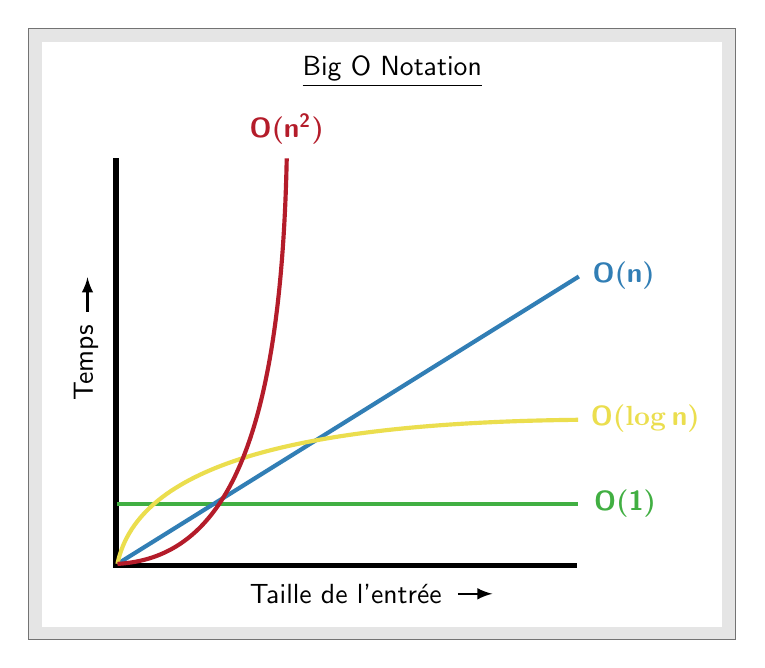
\begin{tikzpicture}[x=1cm,y=1cm,
    font=\sffamily\fontsize{10}{12}\selectfont,
    complexity curve/.style={line width=1.5pt}]
    \definecolor{complexityRed}{RGB}{180,28,42}
    \definecolor{complexityBlue}{RGB}{49,126,181}
    \definecolor{complexityYellow}{RGB}{235,222,78}
    \definecolor{complexityGreen}{RGB}{65,175,66}

    % Same proportions and schematic curves as the original image.
    \path[use as bounding box] (0,0) rectangle (9,7.78);
    \fill[black!10] (0,0) rectangle (9,7.78);
    \fill[white] (0.18,0.17) rectangle (8.82,7.60);
    \draw[black!55,line width=0.4pt]
        (0.01,0.01) rectangle (8.99,7.77);
    \node at (4.63,7.22) {\underline{Big O Notation}};

    \draw[line width=2pt] (1.12,6.12) -- (1.12,0.95) -- (6.98,0.95);
    \node[rotate=90] at (0.74,3.52) {Temps};
    \draw[->,>=latex,line width=0.9pt] (0.76,4.17) -- (0.76,4.61);
    \node (inputSize) at (4.04,0.59) {Taille de l'entrée};
    \draw[->,>=latex,line width=0.9pt] (inputSize.east) ++(0.08,0) -- ++(0.44,0);

    \draw[complexity curve,complexityGreen] (1.14,1.73) -- (6.99,1.73);
    \draw[complexity curve,complexityBlue] (1.14,0.97) -- (7.00,4.62);
    \draw[complexity curve,complexityYellow]
        (1.14,0.97) .. controls (1.40,2.22) and (3.40,2.76) .. (6.99,2.80);
    \draw[complexity curve,complexityRed]
        (1.14,0.97) .. controls (2.38,1.04) and (3.21,2.25) .. (3.29,6.12);

    \node[complexityRed,above] at (3.29,6.17)
        {$\boldsymbol{\mathsf{O(n^2)}}$};
    \node[complexityBlue,right] at (7.05,4.63)
        {$\boldsymbol{\mathsf{O(n)}}$};
    \node[complexityYellow,right] at (7.03,2.81)
        {$\boldsymbol{\mathsf{O(\log n)}}$};
    \node[complexityGreen,right] at (7.07,1.74)
        {$\boldsymbol{\mathsf{O(1)}}$};
\end{tikzpicture}
\end{document}
